\documentclass[12pt,twoside]{scrartcl}
\usepackage[a4paper,top=2cm,left=2cm,right=2cm,bottom=2cm,includefoot,includehead]{geometry}
\usepackage{graphicx}
\usepackage[numbers]{natbib} % Add this line for natbib package
\usepackage{fancyhdr}
\usepackage{hyperref}
\usepackage{amsmath}
\graphicspath{ {figures/} }



\pagestyle{fancy} % Set the page style to fancy
\fancyhf{} % Clear all header and footer fields

% Define the header and footer content for odd and even pages
\fancyhead[CE,CO]{School of Electrical Engineering} % Left header on even pages, right header on odd pages
% \fancyhead[RE,LO]{Right Header} % Right header on even pages, left header on odd pages
\fancyfoot[LE,RO]{\thepage} % Page number on left footer of even pages and right footer of odd pages
\fancyfoot[RE,LO]{ELEC3251} % Left footer on odd pages, right footer on even pages

\begin{document}
\pagenumbering{arabic}
\setcounter{page}{1}
\begin{titlepage}
    \begin{center}

        
\includegraphics[width=0.2\textwidth]{LOGO_Square.pdf}

        \vspace*{0.4cm}
        School of Electrical Engineering \\
        University of Newcastle
        
        \vspace{1cm}
        \huge
        \textbf{\textsf{ELEC3251 \\ Assignment 1}}

        \vspace{0.5cm}
        \large
        \textbf{\textsf{Practical and Theoretical Analysis of \\ Buck Converter and Flyback Converter}}

        \vspace{1.5cm}
        \normalsize
        \begin{tabular}{l|r}
            Liam Patey-Dennis & c3349900 \\
            Joshua Thomas & c3376353
        \end{tabular}
        \vfill    
    \end{center}
\end{titlepage}


\section{Buck Converter}
\subsection{Ideal Calculations}
The duty cycle required to achieve an output voltage of $V_{o} = 5$ V for an input supply voltage of $V_{d} = 12$ V can be determined using the DC transfer function of the Buck converter, see Equation \ref{equation:Buck_TF}. The resulting duty cycle required for the ideal circuit is $D \approx 41.67$\%.\par
\begin{equation}
\frac{V_o}{V_d} = D \label{equation:Buck_TF}
\end{equation}
The output voltage ripple ($\Delta V_o$) of an ideal Buck converter is given by Equation \ref{equation:Buck_ripple}. This equation can be rearranged, see Equation \ref{equation:Buck_cap}, to find the required capacitance for the low pass filter, provided that the duty cycle ($D$), filter inductance ($L$), and switching period ($T_{s}$) are known. For $T_{s} = 1/f_{s} = 10$ $\mu$s, $L = 1$ mH, $D = 41.67$\%, $\Delta V_{o} = 25$ mV, and $V_o = 5$ V, the required capacitance is $C = 1.458$ $\mu$F. \par
\begin{equation}
\frac{\Delta V_{o}}{V_{o}} = \frac{1}{8}\frac{T_{s}^{2}(1-D)}{LC} \label{equation:Buck_ripple}
\end{equation}
\begin{equation}
C = \frac{V_o}{\Delta V_{o}}\frac{T_{s}^{2}(1-D)}{8L} \label{equation:Buck_cap}
\end{equation}
The output power of the converter will be limited by the ratings of the components in the circuit. As the output voltage of the converter is required to remain constant at $5$ V, only the output current can be adjusted to suit the ratings of the components. The inductor selected for the circuit is the Murata \#1410516C, which has a maximum DC current of $1.6$ A \cite{RNX0}. A IRFZ24NPbF MOSFET has been selected for the switch, this component has a maximum DC current rating of $17$ A \cite{RNX1}. The selected diode is an SB120 which has a maximum DC current of $1.0$ A \cite{RNX2}. The inductor current will equal the output current, assuming the voltage across the capacitor remains constant. Therefore, the output current must be less than $1.6$ A, to avoid causing damage to the inductor. The diode will only conduct when the switch is off, therefore the DC current flowing through the diode is $I_{D} = (1-D)I_{o}$. For $I_{o} = 1.6$ A the diode current is $0.93$ A, which is less than the maximum rating of the device. Therefore, the load resistance must be selected such that $I_{o} \le 1.6$ A. Using Ohm’s law this inequality is equivalent to $R_{Load} \ge 3.125$ $\Omega$. The smallest resistor provided in the laboratory kit is $3.9$ $\Omega$ so this resistance will be used for the load.\par
\vspace{5mm}
\noindent The continuous conduction mode (CCM) and discontinuous conduction mode (DCM) boundary occurs when the current flowing through the inductor reaches $0$ A. For the ideal Buck converter this will occur for a DC output current ($I_{oB}$) which can be found using Equation \ref{equation:Buck_DCM}. For the designed converter the minimum DC output current is $I_{oB} = 14.6$ mA, which is equivalent to an output load of $342$ $\Omega$.
\begin{equation}
I_{oB} \approx \frac{T_{s}V_{o}}{2L}(1-D) \label{equation:Buck_DCM}
\end{equation}
\pagebreak
\subsection{Ideal Simulations}
Wolfram System Modeller (Wolfram) was used to simulate the performance of the designed converter. The model used for the simulations is shown in Figure \ref{fig:Buck_idealModel}. The output voltage of the ideal Buck converter is shown in Figure \ref{fig:Buck_idealVout}. The average output voltage, at steady state, is close to 5 V which lies close to the theoretically expected value of 5 V. The slight discrepancy between the simulated value and the expected value may be the result of truncating the duty cycle to 2 decimal places ($5/12 \approx 0.4167$). It may also be a result of the numerical methods used by the Wolfram software to simulate the system. An output voltage ripple of 6.7 mV is observed from the simulations and is shown in Figure \ref{fig:Buck_idealRipple}.\par
\vspace{5mm}
\noindent Figure \ref{fig:buck_DCM} (A) displays the inductor current for a load resistance of 342 $\Omega$. The current reaches a minimum value of $120 $ $\mu$A, which indicates that the converter is close to the CCM-DCM boundary. Figure \ref{fig:buck_DCM} (b) displays the current for a load resistance of 345 $\Omega$. Slight distortion is observed in the waveform near the zero crossing which indicates that the converter has entered DCM. This suggests that the CCM-DCM boundary lies in the range $342 \le R_{Load} \le 345$ $\Omega$ which agrees with the theoretically expected value of 342 $\Omega$. The boundary may not lie exactly at 342 $\Omega$ because of the assumption, made in Equation \ref{equation:Buck_DCM}, that the inductor current and the output current are equal. This assumption is not correct as a small amount of current also flows through the capacitor.

\begin{figure}[h]
    \centering
    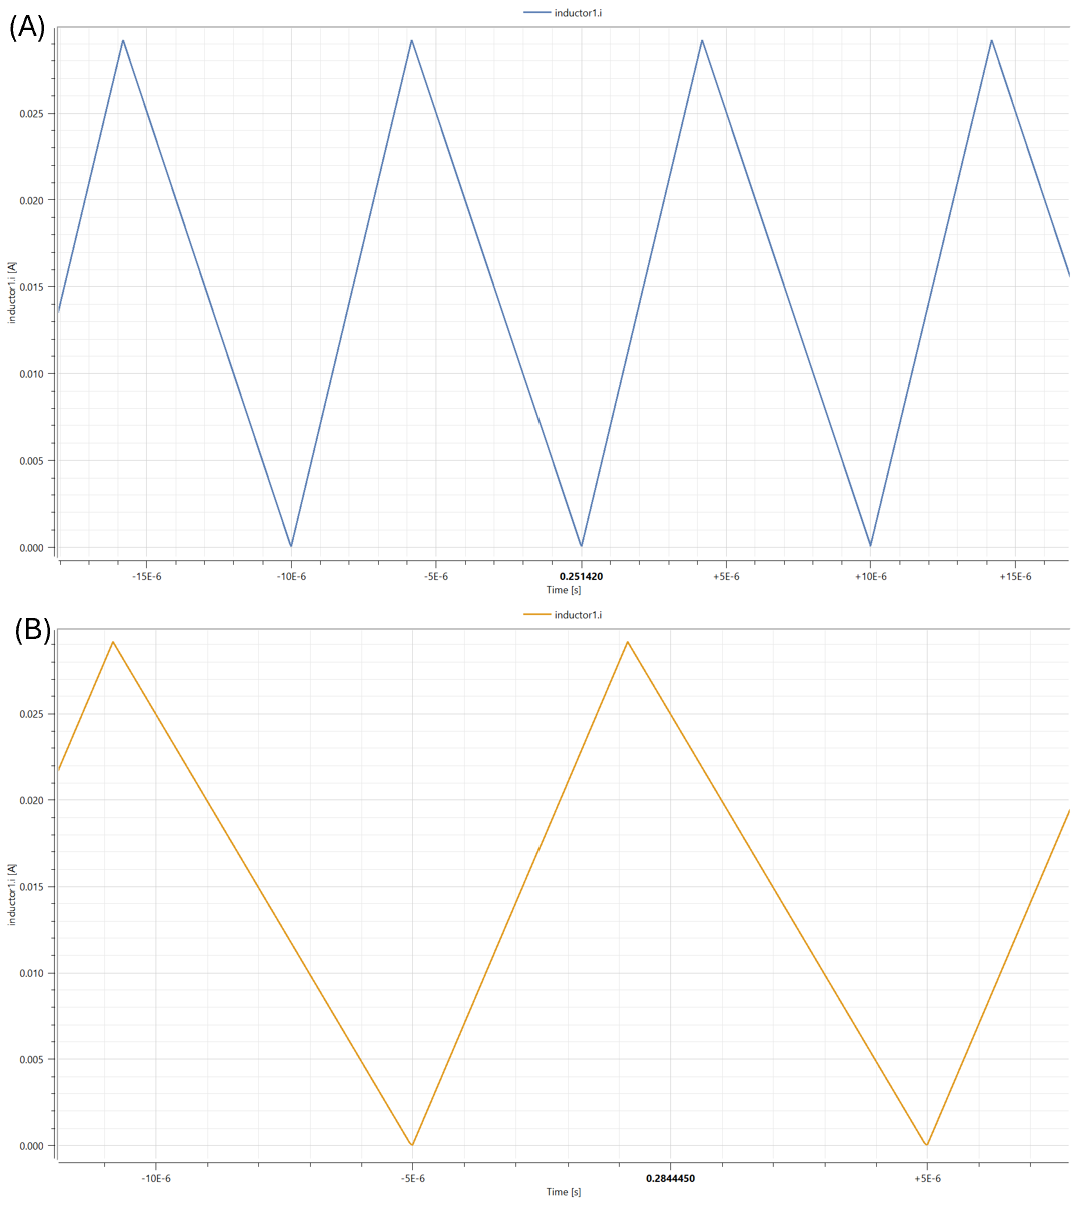
\includegraphics[width=0.6\textwidth]{buck_DCM}
    \caption{Buck converter inductor current for a load resistance of (A) 342 $\Omega$, and (B) 345 $\Omega$. A small amount of distortion is present in (B) which indicates that the CCM-DCM boundary lies in the range $342 \le R_{Load} \le 345$ $\Omega$.}
    \label{fig:buck_DCM}
\end{figure}
\newpage

\subsection{Non Ideal Calculations}
The previous calculations and simulations neglect many real-world effects that will affect the circuit's performance. Previously, no voltage losses were assumed to occur across the switch. This assumption is invalid as real switches are often implemented using transistors that have finite on resistances. Furthermore, it was assumed that no voltage drop occurs across the diode. All diodes have a non-zero voltage drop, which is required to overcome the potential barrier formed at the P-N junction of these devices. In addition, the windings of an inductor are not perfect conductors and hence have resistance. These effects will result in the output voltage of the converter being lower than the theoretically expected value. Figure \ref{fig:Buck_nonIdealCircuits} displays equivalent circuit models which can be used to account for these effects when (A) the switch is on and (B) when the switch is off. Applying Kirchoff’s voltage law (KVL) to the outer loop of each circuit, results in Equations \ref{equation:KVL_on} and \ref{equation:KVL_off}.
\begin{equation}
V_{L,on} = V_{d} - V_{o} - V_{loss, on} = V_{d} - V_{o} - (R_{DS}+ R_{L})i_{L} \label{equation:KVL_on}
\end{equation}
\begin{equation}
V_{L,off} = -V_{o} - V_{f} - V_{loss, off} = V_{o} - V_{f} - R_{L}i_{L}\label{equation:KVL_off}
\end{equation}
Where $R_{DS}$ is the on resistance of the switch, $R_{L}$ is the inductor resistance, and $V_{f}$ is the forward voltage of the diode.\par
\vspace{5mm}
\noindent If it is assumed that the circuit is in steady state, then the zero volt-seconds assumption can be applied which yields,
\begin{equation*}
V_{L,on}t_{on} + V_{L,off}t_{off} = 0
\end{equation*}
If the inductor current is assumed to be equal to the load current then,
\begin{equation*}
i_{L} \approx i_{Load} = \frac{V_{o}}{R_{Load}}
\end{equation*}
Which can be used with the previous equation to obtain Equation \ref{equation:Buck_nonIdealTF}.
\begin{align}
V_{o} &= \frac{R_{Load}}{(1+2D)R_{Load} - R_{L} - DR_{DS}}\left\{DV_{d} - (1-D)V_{f} \label{equation:Buck_nonIdealTF}\right\}
\end{align}
\noindent For the ideal duty cycle ($D = 41.67$\%) with the parameters $R_{DS} = 0.07$ $\Omega$, $R_{L} = 1.6$ $\Omega$, $V_{f} = 0.7$ V and a load current of $i_{L} = 1.28$ A ($R_{Load} = 3.9$ $\Omega$), the expected output voltage of the converter is $V_{o} =3.24$ V \cite{RNX1, RNX0, RNX2}. The duty cycle required to obtain an output of 5 V is $D = 61.44$\%.

INCLUDE EFFECTS OF INDUCTOR TOLERENCE AND LOAD TOLERENCE, MENTION PARASITICS

\newpage
\subsection{Non Ideal Simulations}
The output voltage of the non-ideal converter for the ideal duty cycle is shown in Figure \ref{fig:buck_NI_output_oldD}. Applying a 2nd order low pass filter, with a cutoff frequency of 10 kHz, to the output voltage results in average output voltage of 3.22 V which lies close to the theoretically predicted value of 3.24 V. Figure \ref{fig: buck_NI_output_newD} displays the output voltage for a duty cycle of 61.44 \%, an average voltage of 5.00 V is observed which matches the theoretically predicted value.

\begin{figure}[h]
    \centering
    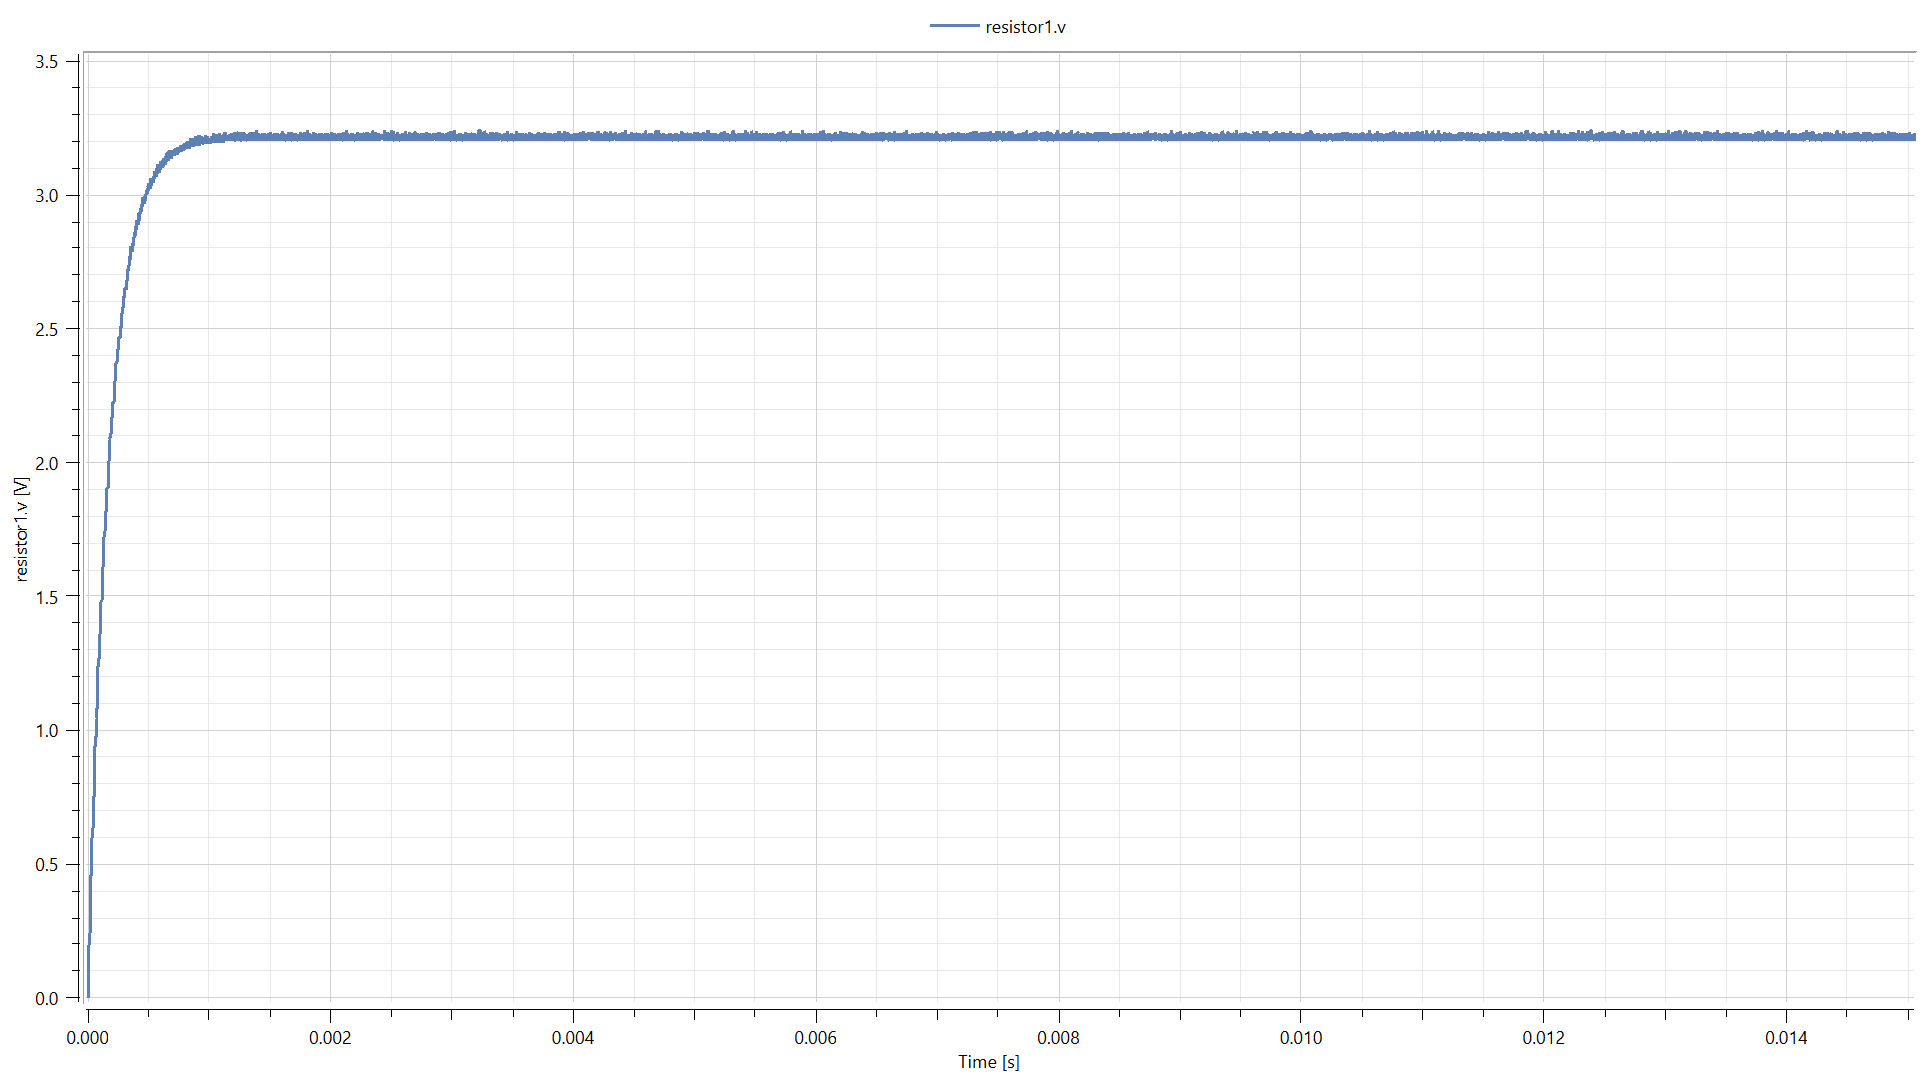
\includegraphics[width=0.6\textwidth]{buck_NI_output_oldD}
    \caption{Non-ideal Buck converter output voltage for duty cycle of 41.67\% and a load of $3.9$ $\Omega$. An average voltage of 3.22 V is observed.}
    \label{fig:buck_NI_output_oldD}
\end{figure}
\begin{figure}[h]
    \centering
    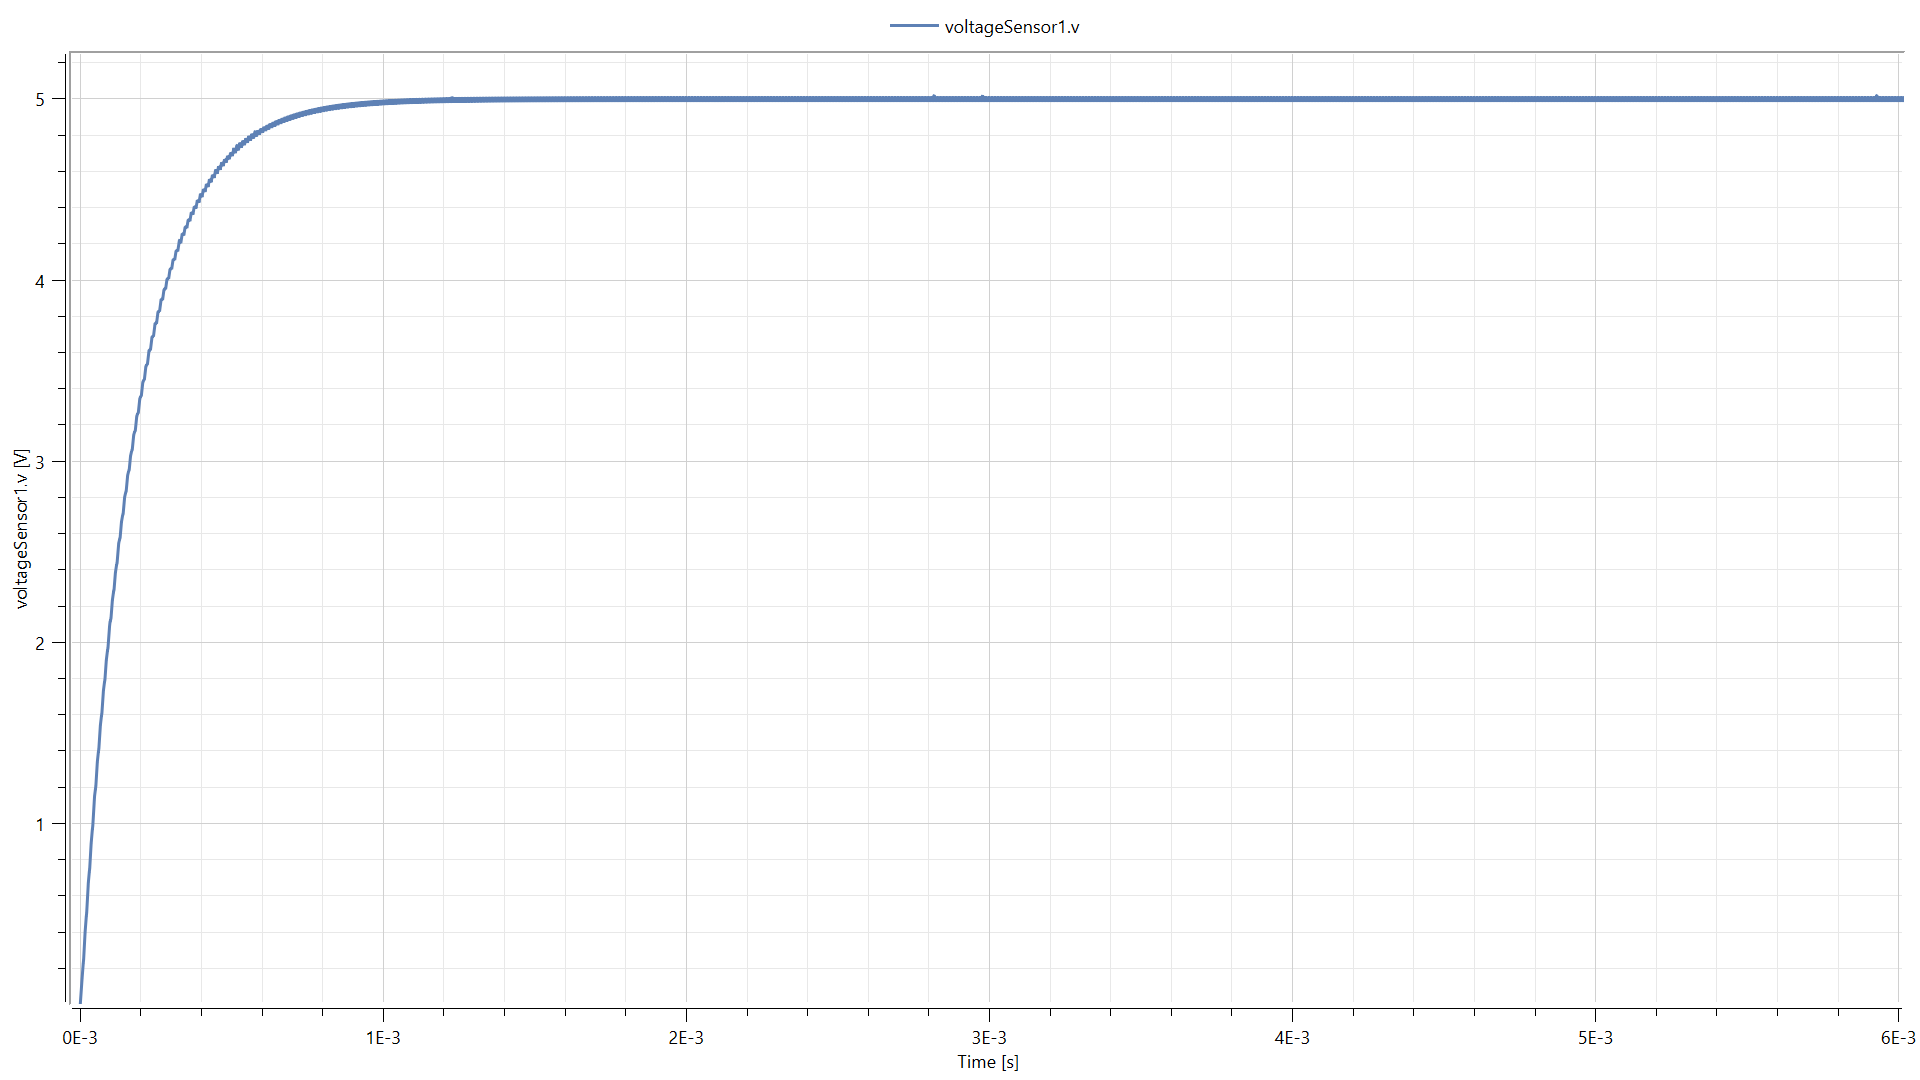
\includegraphics[width=0.6\textwidth]{buck_NI_output_newD}
    \caption{Non-ideal Buck converter output voltage for duty cycle of 61.44\% and a load of $3.9$ $\Omega$. An average voltage of 5.00 V is observed.}
    \label{fig:buck_NI_output_newD}
\end{figure}

\newpage
\section{Flyback Converter}

\newpage
\bibliographystyle{IEEEtranN}
\bibliography{references}

\end{document}
